
\documentclass[12pt,a4paper]{article} 

\pdfoutput=1

\usepackage[T1]{fontenc}
\usepackage[latin9]{inputenc}
\usepackage{verbatim}
\usepackage{float}
\usepackage{amsthm}
\usepackage{amsmath}
\usepackage{amssymb}
\usepackage{graphicx}
%\usepackage{multirow}
\usepackage{color}
\usepackage{url}


\newcommand{\TODO}[1]{{\color{red}{[#1]}}}

\makeatletter


%%%%%%%%%%%%%%%%%%%%%%%%%%%%%% Textclass specific LaTeX commands.
\numberwithin{equation}{section}
\numberwithin{figure}{section}
\theoremstyle{plain}
\newtheorem{thm}{\protect\theoremname}[section]
\theoremstyle{definition}
\newtheorem{defn}[thm]{\protect\definitionname}
\theoremstyle{remark}
\newtheorem{claim}[thm]{\protect\claimname}
\theoremstyle{plain}
\newtheorem{lem}[thm]{\protect\lemmaname}

\newtheorem*{lem*}{Lemma}
\theoremstyle{remark}
\newtheorem{rem}[thm]{\protect\remarkname}
\theoremstyle{plain}
\newtheorem{corollary}[thm]{\protect\corollaryname}
\theoremstyle{plain}
\newtheorem{proposition}[thm]{\protect\propositionname}
%%%%%%%%%%%%%%%%%%%%%%%%%%%%%% User specified LaTeX commands.

%\usepackage{babel}
\providecommand{\claimname}{Claim}
\providecommand{\definitionname}{Definition}
\providecommand{\lemmaname}{Lemma}
\providecommand{\remarkname}{Remark}
\providecommand{\theoremname}{Theorem}
\providecommand{\corollaryname}{Corollary}
\providecommand{\propositionname}{Proposition}


\newcommand{\RL}{\mathbb{R}^L}
\newcommand{\RN}{\mathbb{R}^N}
\newcommand{\CL}{\mathbb{C}^L}
\newcommand{\RNN}{\mathbb{R}^{N\times N}}
\newcommand{\CNN}{\mathbb{C}^{N\times N}}
\newcommand{\inner}[1]{\left\langle {#1} \right\rangle}
\newcommand{\E}[1]{\mathbb{E}\left\{{#1} \right\}}
\newcommand{\order}[1]{\mathcal{O}\left({#1} \right)}
\newcommand{\xz}{x_{\textrm{zp}}}
\newcommand{\DFT}[1]{\operatorname{DFT}\!\left( {#1} \right)}
\newcommand{\hx}{\hat{x}} 


\begin{document}

%\begin{frontmatter}


\title{Multireference alignment meets blind deconvolution}
\author{Tamir Bendory}
\maketitle

\begin{abstract}
	Here comes the abstract
\end{abstract}


\section{Introduction} \label{sec:introduction}

Blind deconvolution is the problem of estimating a signal from its convolution with an unknown kernel. This problem arises in many engineering and scientific applications, such as astronomy, communication, deblurring and optics; see   \cite{jefferies1993restoration,tong1994blind,chan1998total,campisi2016blind,kundur1996blind,levin2011understanding,shalvi1990new,levin2009understanding,krishnan2011blind,ayers1988iterative,michaeli2014blind} to name a few.

Without prior information the blind deconvolution is clearly ill-posed. In this note, we consider a special case of the problem. We aim at estimating a signal $x\in\RL$ from $y\in\RN, \thinspace N\gg L$. The acquired data, the measurement $y$, is composed of many repetitions of $x$, at different positions, and i.i.d.\ normal noise $\varepsilon $with mean zero and variance $\sigma^2$. 
Formally, our model read
\begin{equation}
y[n] = \sum_{i=1}^K \xz [n-n_i] + \varepsilon[n], 
\end{equation}
where $\xz\in\RN$ is a zero-padded version of $x\in\RL$ and 
defined as $$\xz  = [x, \underbrace{0,0,\ldots,0}_{N-L \text{ zeros}}],$$ and
 $n_i,\quad i=1,\ldots,K,$ are the translations of $\xz$.


Note that both $x$ and the translations, or positions, $n_i$ are unknown. Let $s\in\{0,1\}^N$ be the ``support" signal, which takes the value 1 at the locations $n_i$ are zero otherwise. 
Then, 
\begin{equation}
y = \xz \ast s + \varepsilon.
\end{equation}
The goal is then to estimate $x$ from $y$, while $s$ is unknown as well. The support signal $s$ is the latent or hidden variable of the problem. This is quite common in blind deconvolution problem. For instance, in image deblurring, the both the blurring kernel and the high-resolution image are unknown, but the main goal is merely to sharpen the image. In Section~\ref{sec:literature} we survey previous results on blind deconvolution.

Figure~\ref{fig:example} shows examples for the data in different noise levels. In the low noise regime (for instance, the first row), the problem is easy. In this case, one can identify $x$ in $y$ by simple detection algorithms (e.g., thresholding on the correlation function). Once several copies of  signal were detected and cropped from $y$, then one can  improve the SNR by averaging. We are interest in the more challenging regime of high noise level, in which the signal is completely swamped in the noise, and one cannot detect the signal's appearances. In this case, one need to use the prior information that the signal appears many times across the measurement.

\begin{figure}
	\begin{center}
	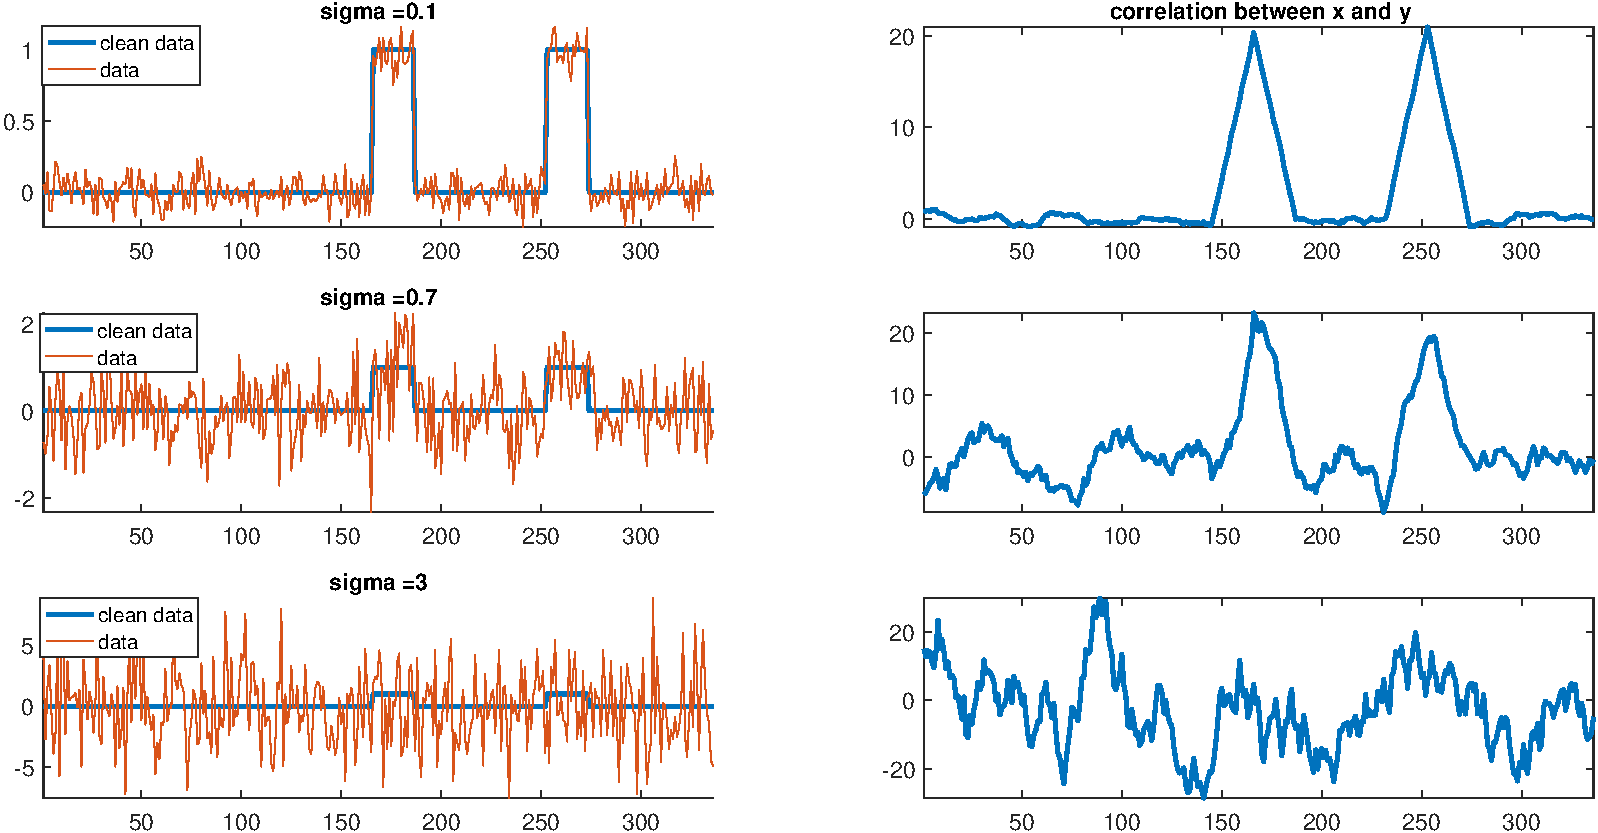
\includegraphics[scale = .4]{example}
	\end{center}
\caption{fdnjfk}
\label{fig:example}
\end{figure}

To perform this blind deconvolution, we use the invariant approach proposed for multireference alignment in a previous paper. Let us  first introduce  notation. We crop the measurement $y\in\RN$ into a series of analysis windows: 
\begin{equation}
y_i = y[(i-1)W + 1 : iW ]\in\mathbb{R}^W, \quad i=1,\ldots,N/W, 
\end{equation}
To ease notation, we assume that  $W$ divides $N$  so that there are exactly $N/W$ windows. We also assume that $\vert n_i - n_j\vert >W$ so that each window contains no more than one signal (in general, we can introduce overlapping windows. The code enables it, but it does not seem to improve performance.).
For each one of the windows, we compute its first three translation-invariant features, namely, mean, power spectrum and bispectrum. We then hope that averaging over these features will produce a reliable estimation of the invariant features of the signal itself. 
We recall that given accurate estimators of those features, we can estimate the signal itself reliably. Therefore, the question boils down to the accuracy of these feature estimations.


\section{Literature survey} \label{sec:literature}


\section{Connection with the cryo--EM problem} \label{sec:cryoEM}
particle picking 

\section{Algorithm} \label{sec:algorithm}


Before moving ahead to the feature estimators, we need to estimate the norm of the signal. This is necessary since many analysis windows do not contain information on the signal, but pure noise. We will use the norm to scale the the signal's estimator.
This can be done as follows. For short, we denote $x_K[n]=\sum_{i=1}^K \xz[n-n_i]$ and note that $\|x_K\|_2^2 = K\|x\|_2^2$. 
Then,
\begin{equation}
\| y\|_2^2 =  \| x_K\|_2^2 + \|\varepsilon\|_2^2 + 2\varepsilon^Tx_K. 
\end{equation}  
As $N\to\infty$, we can estimate 
\begin{equation}
\begin{split}
\E{\| y\|_2^2} &=  \| x_K\|_2^2 + \E{\|\varepsilon\|_2^2} + 2\E{\varepsilon^Tx_K} \\ 
&= K\|x\|_2^2 + N\sigma^2. 
\end{split}	 
\end{equation}   
And therefore, 
\begin{equation}
\|x\|_2^2 \approxeq \frac{\| y\|_2^2 - N\sigma^2}{K}. 
\end{equation}


\section{Analysis} \label{sec:analysis}


Next, we analyze the feature estimation in the asymptotic regime of $N,\sigma,K\to\infty$ and fixed $L,W$. We introduce the ``sparsity factor" defined as $S = \frac{N}{WK}<\infty$, $WK$ is a measure for the ``active" windows. We also define  another zero padded signal $x_W  = [x, \underbrace{0,0,\ldots,0}_{N-W \text{ zeros}}]\in\mathbb{R}^W$.

We want to estimate the features of this signal, and focus on the bispectrum for the sake of simplicity (the estimation of the power spectrum and mean obeys the same methodology). 
In order to estimate the bispectrum we average over the bispectra of the windows, namely, (for the power spectrum, we need to do unbiasing. In addition, we can replace the mean by more robust estimator, like the median.)
\begin{eqnarray}
\hat{B}_{x_W} = \frac{W}{N}\sum_{i=1}^{N/W}B_{y_i}.
\end{eqnarray}
We split the sum into three groups of the windows:
\begin{eqnarray}
\hat{B}_{x_W} = B_\textrm{signal} + B_\textrm{clutter} + B_\textrm{noise}, 
\end{eqnarray}
where
\begin{itemize}
	\item $B_\textrm{noise}$ - sum of the bispectra of the segments that contain pure noise (no signal),
	\item $B_\textrm{signal}$ - sum of the bispectra of the segments that contain a full signal (one appearance of $x$) and noise,
	\item $B_\textrm{clutter}$ - sum of the bispectra of the segments that contain only part of $x$ and noise.
\end{itemize}

We first observe that $B_\textrm{noise}\to 0$ (note that this is the zero matrix). More precisely, the variance of the noise goes to zero at rate  $\order{\frac{W}{N}\left(1-\frac{1}{S}\right)\sigma^6}$. In addition, under the assumption that $n_i$ (if appear) are distributed uniformly in the window (we need to come up with precise statistical model; but it would be rather easy), there are (asymptotically) $K(1-L/W)$ windows with complete signals. Therefore,
$B_\textrm{signal}\to \frac{KW(1-L/W)}{N}B_x$ at rate $\order{\frac{\sigma^6}{K(1-L/W)}}$. (Here we need to be a bit careful with the mean of the signal, or to assume it is zero.) Note that the scaling would be corrected at the last stage of the algorithm, by rescaling according to the estimated  norm.

The more interesting term is the ``clutter" --- the cropped signals. Since each such signal appears in two windows,
we have $2KL/W$ clutter segments. Of course, the noise in this segments goes to zero
at rate $\order{\frac{W\sigma^6}{2KL}}$. However, we have an additional error term arises from  the cropped signals. To analyze the effect of this term, let us assume that $N/\sigma^6$ is great enough so that $B_\textrm{noise}\to 0$. Then,
\begin{equation}
\begin{split}
\left\| \hat{B}_{x_W} - B_\textrm{signal}\right\|_{\textrm{F}} \approxeq&  \left\|B_\textrm{clutter}\right\|_{\textrm{F}}
= \left\|\frac{W}{N}\sum_{i\in\textrm{clutter}}B_{y_i}\right\|_{\textrm{F}}
\\ \leq & 
\frac{W}{N}\frac{2KL}{W}\left\|B_x\right\|_{\textrm{F}} = \frac{2L}{SW}
\|B_x\|_{\textrm{F}}.
\end{split}
\end{equation}
Therefore, for large sparsity term $S$ or large $W/L$, we get an accurate estimation of a scaled version of the signal's bispectrum. 


Few insights from the analysis: (need to check numerically)
\begin{itemize}
	\item Larger $S$ reduces the clutter error, however, increases the variance of the noise estimation.
	\item Larger $W/L$ reduces the clutter error, however, increases the variance of the noise  of $B_\textrm{noise}$.
	\item We must keep $W/L$ large enough to see enough full signals.    
\end{itemize} 




\section{Conclusion} \label{sec:conclusion}




\bibliographystyle{plain}
\bibliography{ref}

\end{document}


 